\label{chap:JapanDataset}

\section{Why we chose the Japanese Economy}

Past research shows a major focus on bankruptcy prediction models for the American and European market.
In an attempt to contribute to research focused on the Asian market, we focus our attention to Japan - one of the largest economies in the world. As of 2018, the market capitalisation\footnote{Market capitalisation (also known as market value) is the share price times the number of shares outstanding (including their several classes) for listed domestic companies.} of Japan is the third-largest in the world at \textbf{\$5.296 trillion} (\href{https://www.world-exchanges.org/our-work/statistics}{Source: World Federation of Exchanges database}), with the US and China having the largest global markets values respectively. Countries like the United Kingdom, Germany and France are similar to most capital markets but are significantly different from the countries in Asia.

\begin{figure}[htpb]
\centering
\frame{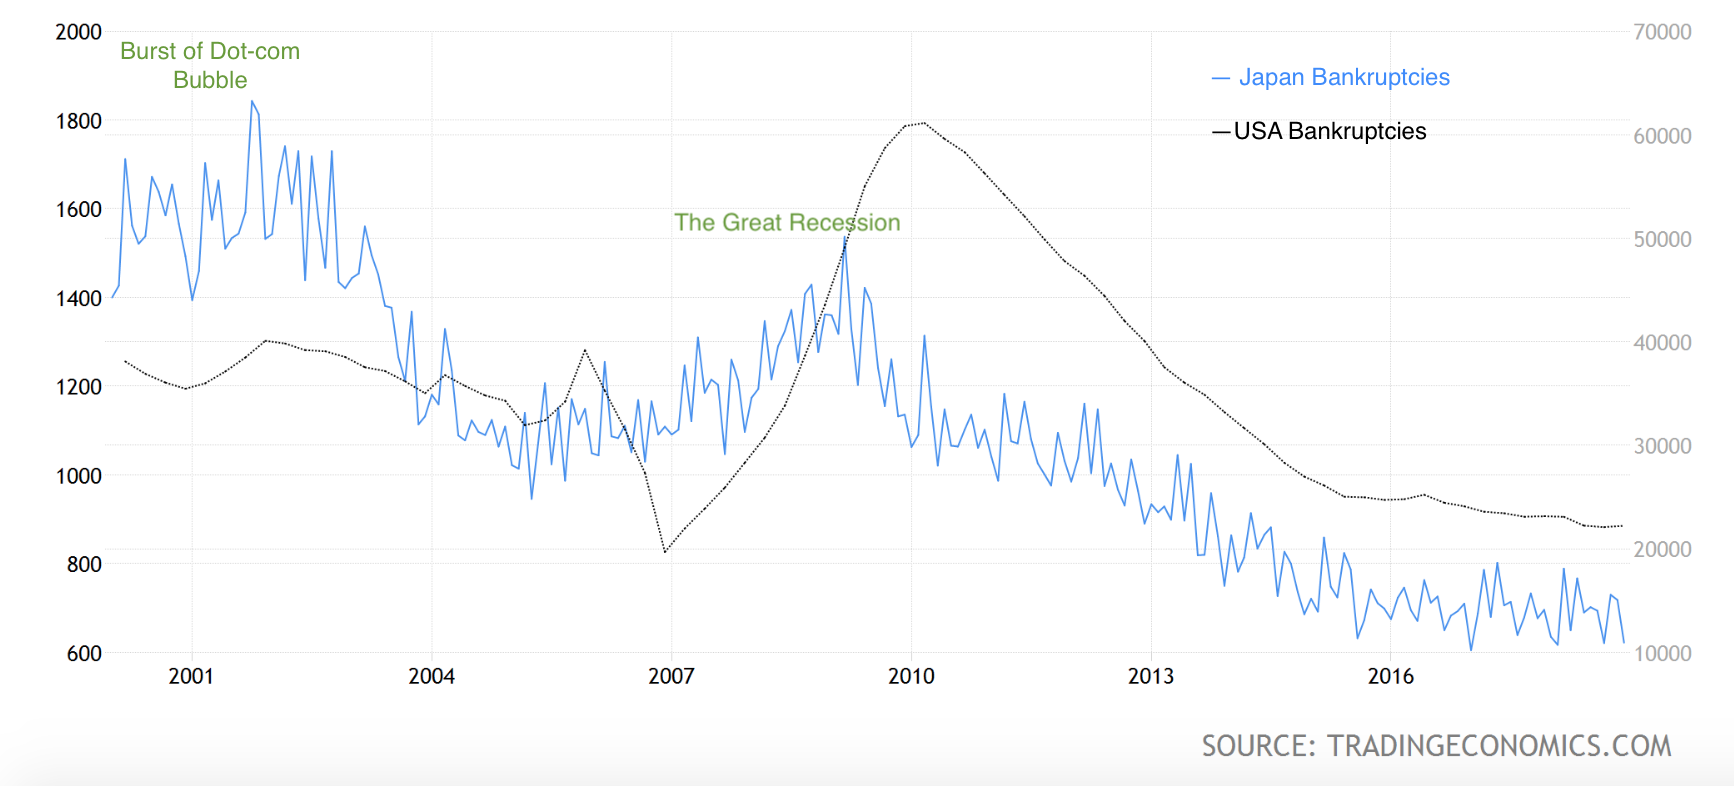
\includegraphics[height=5cm,width=\columnwidth]{Images/usaVsJapan.png}}
\caption{Comparing the number of bankruptcies in Japan and USA between 2000-2018. Source:\href{https://tradingeconomics.com/japan/bankruptcies}{ Trading Economies} }
\label{Fig:japUSA}
\end{figure}
% Location-wise, UK, Germany, France and Japan are among the leading economies in Europe and Asia. 

A comparison between Japan and the US in the number of corporate bankruptcies between 2000-2018 can be seen in \autoref{Fig:japUSA}. The figure summarises the number of bankruptcy filings each year and it is clear that the bankruptcy filing events display a strong cyclical trend. In specific, we can note the two big jumps around the most recent global recession periods, namely, the early 2000s and late 2000s. Such business-related fluctuation confirms the existence of the “domino-effect” financial distress at an international level.

In Japan, the two most prominent legal routes for filing for bankruptcy are: filing for court protection from creditors under the Corporation Reorganisation Law or under the Civil Rehabilitation Law.

The Corporation Reorganisation Law is aimed at firms whose failure would have a big impact on society, the management must resign and a new team is brought in according to a reorganisation plan devised by a court-appointed administrator. Although this procedure allows the company to sever ties with executives deemed responsible for the collapse, recovery often takes longer under this process than via the Civil Rehabilitation Law.
The Civil Rehabilitation Law, similar to America's Chapter 11, is often preferred because it allows the company to rebuild under its management team, speeding up the reconstruction process.

\section{Data-source}
\label{sec:dataSource}
We obtained the financial data of 4000 Japanese firms from an international financial database, provided by Wharton Research Data Services (\href{https://osiris.bvdinfo.com/version-20191113/home.serv?product=OsirisNeo}{Website: WRDS}). WRDS ensures convenient comparability among different countries without loss of the data consistency and reliability, regardless of differences in geometric location, business regulations etc. The database has information on listed, and major unlisted/delisted, companies across the globe. Japanese corporations also have well documented financial data as they adopt GAAP\footnote{Generally accepted accounting principles (GAAP) refer to a common set of accounting principles, standards, and procedures issued by the Financial Accounting Standards Board (FASB).} for consolidated financial statements.
% The information is very detailed and includes a lot more than financial reports.

To formally construct the international bankruptcy database, we collected each firm's annual financial information and its bankruptcy status from WRDS' annual files, this includes data from the Tokyo Stock Exchange and Osaka Securities Exchange.

% In Japan, there are six ways (including two out-of-court procedures) for a business to pursue bankruptcy proceedings. The two most prominent legal routes are: filing for court protection from creditors under the Corporation Reorganisation Law or under the Civil Rehabilitation Law.

% The Corporation Reorganisation Law is aimed at firms whose failure would have a big impact on society, the management must resign and a new team is brought in according to a reorganisation plan devised by a court-appointed administrator. Although this procedure allows the company to sever ties with executives deemed responsible for the collapse, recovery often takes longer under this process than via the Civil Rehabilitation Law.
% The Civil Rehabilitation Law, similar to America's Chapter 11, is often preferred because it allows the company to rebuild under its management team, speeding up the reconstruction process.

% When a company folds, there are two court procedures to follow: filing for bankruptcy protection or filing for special liquidation when the entity has excessive debts. 
% A company is generally deemed bankrupt if it dishonours checks twice in six months.
To maintain comparability with other studies, we have chosen to adopt the following definition of bankruptcy - a firm is classified as “bankrupt” if it files either Chapter 7 (liquidation) or Chapter 11 (using the Civil Rehabilitation Law). 
In particular, the bankruptcy indicator for the firm `i' at a time `t' is set to 1 if the firm was delisted due to filing for Chapter 7 or Chapter 11, at the time `t'. There are very few cases that firms who were delisted may re-enter the database later, but we do not consider any firm's observation after their first delisting in our analysis. 
% Companies that exit from the database for other reasons are considered as “non-bankruptcy” firms.

\subsection{Choosing 2000 to 2018 as a Sampling Period}
\label{sec:financialHistory}
In this study, we have chosen to limit our sampling period to begin from 2000 to 2018 as the Japanese economy went underwent a series of changes in bankruptcy regulations in the years leading up to 2000.
In 1998, the Japanese financial regulatory standard was tightened by the government \cite{nakamura2006japanese}. Doing so greatly weakened the original corporate structure of Japanese market - a system that mainly relied on the connection to the main bank and/or the major Keiretsu\footnote{A keiretsu is a set of companies with interlocking business relationships and shareholdings. In the legal sense, it is a type of informal business group that are loosely organised alliances within the social world of Japan's business community.} groups for financing; The research in \cite{xu2009bankruptcy} showcases this in further detail. 
Before 1998, a firm that was unable to pay off the debt from its creditors could seek financial support from the "main bank" or a certain Keiretsu group, if the company was associated to any, to avoid stepping in any further default filing process. However, after the government tightened the regulatory standard, neither the main bank nor the Keiretsu group was allowed to save a firm from default. This institutional structure change leads to an increased number of bankruptcy filings. Therefore, to avoid skewed bankruptcy figures, we begin our sampling only from 2000. 


\section{Dataset Reorganisation}
Re-organising the dataset was the most time-consuming task and the hardest challenge that we faced. The initial WRDS data set consisted of financial data from 1990 to 2018 of 4000 Japanese firms. Accounting for the reasons mentioned in the above sub-section, we first removed all the data that predated 2000. 
Our next big challenge was to combine all the available information on one timescale, as not all companies followed GAAP standards of reporting data. Careful and precise efforts needed to be undertaken to ensure that all financial indicators were reported in the same month/year so that further examinations could be made.

Acknowledging that financial data suffers from class imbalance\footnote{Our dataset consists of bankrupt and non-bankrupt/operational companies. The number of companies that go bankrupt is far fewer than the number of companies that remain operational, hence a company that goes bankrupt is part of the minority class} and concept drift\footnote{Concept drift has been explained in detail in Appendix \autoref{conceptDrift}.} that results in poor and degrading predictive performance in predictive models.  This paper proposes the use of rolling time window (as recommended in \cite{molodtsova2009out,huang2012dynamic,stock2007has}) with a fixed window size. 

% Sun \cite{sun2010dynamic} studied the mechanism of rolling time windows with fixed and variable widths, and their results showed that there was a certain degree of concept drift in financial distress prediction of Chinese listed companies. That is, under the unchanging standard definition of financial distress, incremental data would gradually take on new features of corporate financial distress in a new economic environment with time past. 

Building on the successes seen in \cite{matsunaga2019exploring,li2019dp,molodtsova2009out}, we have decided to incorporate a ten-year rolling window, to predict bankruptcy in a one-year horizon. This required us to reorganise the data to represent five forecasting years, i.e, Year 1, Year 2, Year 3, Year 4 and Year 5. This approach has been explored to outperform conventional bankruptcy models that otherwise use data from a fixed period to predict bankruptcy within a fixed horizon (number of years). \autoref{table:rolling Window} showcases the steps we have taken to reorganise the dataset, to carry out a prediction task.

\begin{table}[h!]
\begin{center}
%  \begin{tabular}{|p{2cm}|p{3cm}|p{3cm}|p{3cm}|}
 \begin{tabular}{|c|c|c|c|}
\hline
 Dataset Name & Prediction Year & Window Length & Number of Firms in Dataset 

  \\ [0.5ex] 
\hline\hline
 
Year 1 & 2013 & 2003 - 2012 & 2342  \\ \hline
Year 2 & 2014 & 2004 - 2013 & 3391  \\ \hline
Year 3 & 2015 & 2005 - 2014 & 3501  \\ \hline
Year 4 & 2016 & 2006 - 2015 & 3264  \\ \hline
Year 5 & 2017 & 2007 - 2016 & 1970  \\ 
\hline
\end{tabular}
\end{center}

    \caption{Using rolling windows to predict the bankruptcy in the next financial year.}
\label{table:rolling Window}
\end{table}


% \begin{table}[h!]
% \scriptsize
% % \captionsetup{font=normal}
% \setlength\defaultaddspace{0.66ex}
% \centering
% \begin{threeparttable}
  
%   \label{tab:history}%
%     \begin{tabular}{|l|l|l|l|}
%     \toprule
%     \textbf{Dataset Name} & \textbf{Prediction Year} & \textbf{Window Length} & \textbf{Number of Firms in Dataset}  \tabularnewline
%     \midrule
%     Year 1 & 2013 & 2003 - 2012 & 2342  \tabularnewline
% \addlinespace
%     Year 2 & 2014 & 2004 - 2013 & 3391  \tabularnewline
% \addlinespace
%     Year 3 & 2015 & 2005 - 2014 & 3501  \tabularnewline
% \addlinespace
%     Year 4 & 2016 & 2006 - 2015 & 3264  \tabularnewline
% \addlinespace
%     Year 5 & 2017 & 2007 - 2016 & 1970  \tabularnewline
% \addlinespace
    
% %     1878 & Bernard & Physiological state of cells can be maintained after the death of an organism \tabularnewline
% % \addlinespace
% %     1885 & Roux & Maintained chick embryonic cells in warm salt solutions \tabularnewline
% % \addlinespace
% %     1989 & Amgen Inc. & Recombinant erythropoietin produced in CHO cells \tabularnewline
%     \bottomrule
%     \end{tabular}%
%     \caption{Historical milestones in development of animal cell cultures (\cite{butler2004, verma2014})}
% \end{threeparttable}
% \end{table}%


\section{Dataset Description}

\subsection{Feature Extraction: Using Financial Ratios}

Studies in the past have aimed at proposing novel machine learning techniques to enhance the models’ prediction performances. However, research focused on the effect of the input variables (or features) on prediction performance is scarce.
In general, financial ratios (FRs) have been recognised as one of the most important factors affecting bankruptcy prediction and are used to develop prediction models \cite{Altman,beaver1967financial,ohlson1980financial}.

Our feature selection is based on the seminal papers \cite{Altman,beaver2005have,hardle2009variable,tian2017financial,tian2015variable, ding2012class}. A comprehensive use of financial ratios in bankruptcy prediction can be seen in the study \cite{liang2016financial}.
Financial ratios generally cover seven categories, which reflect the company’s solvency, profitability, cash flow ratios, capital structure ratios, turnover ratios, company growth and others.

%Why chosen those features
Our feature selection for this project was done by taking a tailored combination of the top eighty, most frequently occurring financial ratios that have been used in the above-mentioned papers.
% We have taken a tailored combination of the features from the above mentioned papers, based on their frequency of use and their relevancy. We chose a selection of the 100 most frequently occurring financial ratios that we deemed were important based of past literature. 
For this purpose, our Japanese dataset was re-structured to create these eighty financial ratios. In doing so, we realised that our dataset had a few limitations as it did not contain data related to the ownership structures\footnote{Ownership structure data mainly involves data related to shareholders i.e., the shareholding ratio of the board, shareholding ratio of directors, shareholding ratio of an outside person, etc.},  turnover of  `C-level' executives and compensation given to board members.
% \todo{Can be in future work - incl employee compensation}

Discarding these financial ratios, we were able to create sixty-four financial ratios that could be used as predictive variables. These synthetic features were generated by a selection of two or more existing features and applying an arithmetical operation on them. The arithmetic operation included the following set of possible values: $\{{+,-, \times,\div}\}$.

% As the focus in our project is the use of ensemble models, we use tree-based models as they have shown effective learning from the data described by many features \cite{zhou2014bankruptcy}. 

The central idea we have used in our approach is to leverage financial ratios as they may have a better influence on prediction than typical economic factors \cite{liang2016financial}. Combining financial ratios with the use of tree-based ensemble models has resulted in more effective learning from the data as shown in \cite{zhou2014bankruptcy}. We have taken advantage of this property and further propose a model that uses an ensemble of boosted trees, dedicated to solving the problem of bankruptcy prediction. 

% We can then evaluate the popularity of each feature in the forest by calculating the total number of occurrences in trees that constitutes the forest. Let us denote the total number of occurrences of
% the $d$ -th feature in the forest structure by $m_{d} .$ We define the categorical distribution $\boldsymbol{\theta}_{F}=\left[\theta_{F}^{(1)}, \cdots, \theta_{F}^{(d)}, \cdots \theta_{F}^{(D)}\right]$ for selecting the features to be
% replicated in the following manner:

% \begin{equation}
% \theta_{F}^{(d)}=\frac{m_{d}}{\sum_{d=1}^{D} m_{d}}
% \end{equation}

% As a consequence, the most popular features are going to be selected for reproduction (by the base learners in the ensemble models). The proposed procedure can be seen as a kind of an evolutionary approach that selects the strongest parents for the child feature.

The research done by Beaver, McNichols, and Rhie in \cite{beaver2005have}, on global markets, concluded that over a long period of time, the performance of the bankruptcy prediction model with both financial statement data and market data is essentially similar to the one with financial ratios only. Therefore we have considered only FRs in our model.

A description of the sixty-four features is presented in \autoref{table:FRstatsDefault}. All variables used for calculation of the financial indicators are obtained from the balance sheets, income statements or cash flow statements of the companies.


\begin{table}
\begin{center}
\small
 \begin{tabular}{|p{0.65cm}|p{6.5cm}|p{0.65cm}|p{6.5cm}|} 
\hline
 ID  & Description & ID  & Description \\ [0.5ex] 
\hline\hline
 
    X1 & Net Profit / Total Assets & X33 & Operating Expenses / Short-Term Liabilities \\ \hline

    X2 & Total Liabilities / Total Assets & X34 & Operating Expenses / Total Liabilities \\ \hline

    X3 & Working Capital / Total Assets & X35 & Profit on Sales / Total Assets \\ \hline

    X4 & Current Assets / Short-Term Liabilities & X36 & Total Sales / Total Assets \\ \hline

    X5 & [(Cash + Short-Term Securities + Receivables - Short-Term Liabilities) / (Operating Expenses - Depreciation)] * 365 & X37 & (Current Assets - Inventories) / Long-Term Liabilities \\ \hline

    X6 & Retained Earnings / Total Assets & X38 & Constant Capital / Total Assets \\ \hline

    X7 & EBIT / Total Assets & X39 & Profit on Sales / Sales \\ \hline

    X8 & Book Value of Equity / Total Liabilities & X40 & (Current Assets - Inventory - Receivables) / Short-Term Liabilities \\ \hline

    X9 & Sales / Total Assets & X41 & Total Liabilities / ((Profit on Operating Activities + Depreciation) * (12/365)) \\ \hline

    X10 & Equity / Total Assets & X42 & Profit on Operating Activities / Sales \\ \hline

    X11 & (Gross Profit + Extraordinary Items + Financial Expenses) / Total Assets & X43 & rotation Receivables + Inventory Turnover in Days \\ \hline

    X12 & Gross Profit / Short-Term Liabilities & X44 & (Receivables * 365) / Sales \\ \hline

    X13 & (Gross Profit + Depreciation) / Sales & X45 & Net Profit / Inventory \\ \hline

    X14 & (Gross Profit + Interest) / Total Assets & X46 & (Current Assets - Inventory) / Short-Term Liabilities \\ \hline

    X15 & (Total Liabilities * 365) / (Gross Profit + Depreciation) & X47 & (Inventory * 365) / Cost of Products Sold \\ \hline

    X16 & (Gross Profit + Depreciation) / Total Liabilities & X48 & EBITDA (Profit on Operating Activities - Depreciation) / Total Assets \\ \hline

    X17 & Total Assets / Total Liabilities & X49 & EBITDA (Profit on Operating Activities - Depreciation) / Sales \\ \hline

    X18 & Gross Profit / Total Assets & X50 & Current Assets / Total Liabilities \\ \hline

    X19 & Gross Profit / Sales & X51 & Short-Term Liabilities / Total Assets \\ \hline

    X20 & (Inventory * 365) / Sales & X52 & (Short-Term Liabilities * 365) / Cost of Products Sold) \\ \hline

    X21 & Sales (n) / Sales (n-1) & X53 & Equity / Fixed Assets \\ \hline

    X22 & Profit on Operating Activities / Total Assets & X54 & Constant Capital / Fixed Assets \\ \hline

    X23 & Net Profit / Sales & X55 & Working Capital \\ \hline

    X24 & Gross Profit (in 3 years) / Total Assets & X56 & (Sales - Cost of Products Sold) / Sales \\ \hline

    X25 & (Equity - Share Capital) / Total Assets & X57 & (Current Assets - Inventory - Short-Term Liabilities) / (Sales - Gross Profit - Depreciation) \\ \hline

    X26 & (Net Profit + Depreciation) / Total Liabilities & X58 & Total Costs /Total Sales \\ \hline

    X27 & Profit on Operating Activities / Financial Expenses & X59 & Long-Term Liabilities / Equity \\ \hline

    X28 & Working Capital / Fixed Assets & X60 & Sales / Inventory \\ \hline

    X29 & Logarithm of Total Assets & X61 & Sales / Receivables \\ \hline

    X30 & (Total Liabilities - Cash) / Sales & X62 & (Short-Term Liabilities *365) / Sales \\ \hline

    X31 & (Gross Profit + Interest) / Sales & X63 & Sales / Short-Term Liabilities \\ \hline
    
    X32 & (Current Liabilities * 365) / Cost of Products Sold & X64 & Sales / Fixed Assets \\ \hline
\end{tabular}
\end{center}
    \caption{Summary of features used}
\label{table:FRstatsDefault}
\end{table}


\subsection{Data Range and Correlations}
% The data ranges including the Min, Max and Mean for each financial ratio, for all 5 years can be seen in Appendix \autoref{sec:dataRange}. 

Appendix \autoref{sec:dataRange} contains the data ranges including the minimum, maximum and mean values of the financial ratios. We present the data ranges for each window (Year 1, Year 2, Year 3, Year 4 and Year5).
We have also included correlation heatmaps for the FRs in Appendix \autoref{sec:corrHeat}, examining these heatmaps, we conclude that we have a good degree of variability in our features as the heatmaps show a low correlation between features.

\subsection{Handling Missing Data}

There are three typical mechanisms causing missing data \cite{little2012prevention,sterne2009multiple,dziura2013strategies}: 
\begin{enumerate}
    \item Missing completely at random (MCAR)
    \item Missing at random (MAR)
    \item Missing not at random (MNAR)
\end{enumerate}

If the mechanism causing missing data is not dependent on observed data nor on the missing data, then data is said to be missing completely at random (MCAR) \cite{sterne2009multiple,dziura2013strategies}. MCAR causes enlarged standard errors due to the reduced sample size but do not cause bias (‘systematic error’ that is an overestimation of benefits and underestimation of harms). 
% In this situation, the incomplete data-sets are representative for the entire dataset \cite{sterne2009multiple}. More often the mechanism of missingness may depend on the observed data. If it only depends on the observed data, then the missing data are missing at random (MAR) given the observed data . 
The MAR and MNAR conditions cannot be distinguished based on the observed data since,  by definition missing data are unknown and it can therefore not be assessed if the observed data can predict the unknown data \cite{sterne2009multiple,dziura2013strategies}.


% % https://www.sciencedirect.com/science/article/pii/S095741741830616X
As justified in \cite{hosaka2019bankruptcy}, missing values in Japanese financial data could be due to the following reasons:
\begin{enumerate}
    \item The Japanese accounting standards for the net assets section changed in 2006.
    \item The notation for accounting items can differ depending on the industry, even if they have similar meanings.
    \item Items that have zero value are missing. This might cause erroneous calculations when computing financial ratios.
\end{enumerate}

Conducting further exploratory data analysis (after having created our financial ratios), we found that the dataset still contained several missing values. Examining this more closely, the dataset was tested to observe the extent of data loss if listwise deletion (an entire record is excluded from analysis if any single value is missing) is used. We observe that the data loss would be severe as we lose over 50\% of our available data. This is detailed in \autoref{table:dataLoss}

\begin{table}[h!]
% \sma
\begin{center}
 \begin{tabular}{|l|p{2.75cm}|p{2.75cm}|p{2.75cm}|p{2.75cm}|} 
 
\hline
 Dataset  & Total number of instances & Number of instances with missing data & Number of instances with no missing data & Data loss if listwise deletion is used
  \\ [0.5ex] 
 \hline\hline
 
Year 1 & 2342 & 1278 & 1064 & 54.54\% \\ \hline
Year 2 & 3391 & 2029 & 1362 & 59.81\% \\ \hline
Year 3 & 3501 & 1879 & 1628 & 53.48\% \\ \hline
Year 4 & 3264 & 1675 & 1589 & 51.29\% \\ \hline
Year 5 & 1970 & 960 & 1010 & 48.71\% \\ \hline
\hline

\end{tabular}
\end{center}

    \caption{Data Quality Assessment: Missing Data}
\label{table:dataLoss}
\end{table}

Furthermore, the python library \textbf{missingno} was used to visualise the features that had missing values. Nullity matrices were created for each forecasting period to find visual patterns of missing values; white spaces in the graph can be inferred as missing values. An example of the Year 2 dataset can be seen in \autoref{Fig:nullMatrix}

\begin{figure}[htp]
\centering
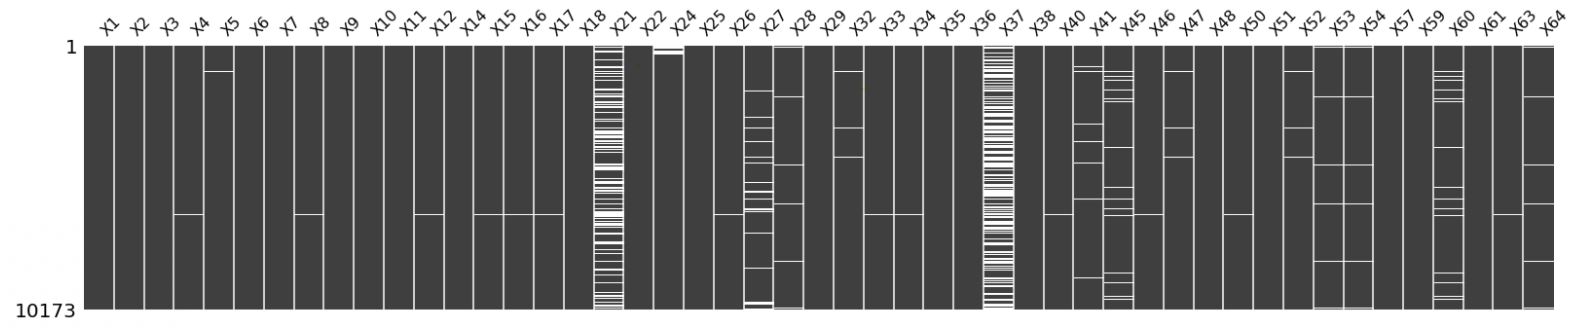
\includegraphics[height=5cm,width=1.0\columnwidth]{Images/nullityMatrix.png}
\caption{Nullity Matrix for Year 2. White space along a feature column represents missing data.}
\label{Fig:nullMatrix}
\end{figure}


In an attempt to make the data richer, we have removed all those instances that have over 50\% of their attributes as either `n.a.' or blank/empty - this resulted in our dataset shrinking by 10.3 \%. 
% This is why the number of instances is lower than expected. In doing so, the Year 5 dataset has the largest impact as the total number of available instances is reduced to 1970 as seen in \autoref{table:rolling Window}. 

Missing data can potentially cause three major problems \cite{kang2013prevention}:
\begin{enumerate}
    \item The missing data can cause bias in the estimation of parameters.
    \item It can reduce the representativeness of the samples and may complicate the analysis of the study.
    \item The absence of data reduces statistical power, which refers to the probability that the test will reject the null hypothesis when it is false.
\end{enumerate}

Dropping all the rows with missing values or listwise deletion introduces bias and affects representativeness of the results. A viable alternative to listwise deletion is by estimating missing data by using imputation techniques. In our project, we explored three techniques of imputation, and we will see them in the subsequent sections.

\begin{enumerate}
    
    
    \item Expectation-Maximisation Imputation
    \item k-Nearest Neighbours Imputation
    \item Multivariate Imputation Using Chained Equations
\end{enumerate}

% ----------------------        EM Imputation     -----------

\subsection{Expectation-Maximisation Imputation}
In statistics, Expectation–Maximisation (EM) is an iterative method to find maximum likelihood estimates of parameters in statistical models. The EM iteration alternates between performing an expectation (E) step, which creates a function for the expectation of the log-likelihood evaluated using the current estimate for the parameters. This is followed by a maximisation (M) step, which computes parameters maximising the expected log-likelihood found on the E step \cite{musil2002comparison}. 
These parameter-estimates are then used to determine the distribution of the latent variables in the next E step. 
EM Imputation is, therefore, the process of imputing missing values using Expectation-Maximisation. Missing values of quantitative variables are replaced by their expected value computed using the Expectation-Maximisation (EM) algorithm. 
In practice, a Multivariate Gaussian distribution is assumed. In general, EM imputation is better than mean imputations because they preserve the relationship with other variables \cite{ambler2007comparison}. 

We carried out EM Imputation using python's \textit{impyute} library and used 50 as the number of EM iterations to run before breaking.

% ----------------------        KNN Imputation     -----------

\subsection{k-Nearest Neighbours Imputation}

The k-nearest neighbour's algorithm or kNN is a non-parametric method used for classification and regression. In both cases, the input consists of the k closest training examples in the feature space. It can also be used as a data imputation technique where kNN imputation replaces `n.a.' and empty values in the data with the corresponding value from the nearest-neighbour row. The nearest-neighbour row is the closest row by Euclidean distance. If the corresponding value from the nearest-neighbour is also `n.a.', the next nearest neighbour is used. After finding k nearest neighbours, the weighted average of them is returned.

We carried out kNN Imputation using python's \textit{fancyimpute} library and used 100 nearest neighbours for the process.



% ----------------------        MICE Imputation     -----------

\subsection{Multivariate Imputation using Chained Equations}

\begin{figure}[htp]
\centering
\captionsetup{justification=centering}
  
  \centering
    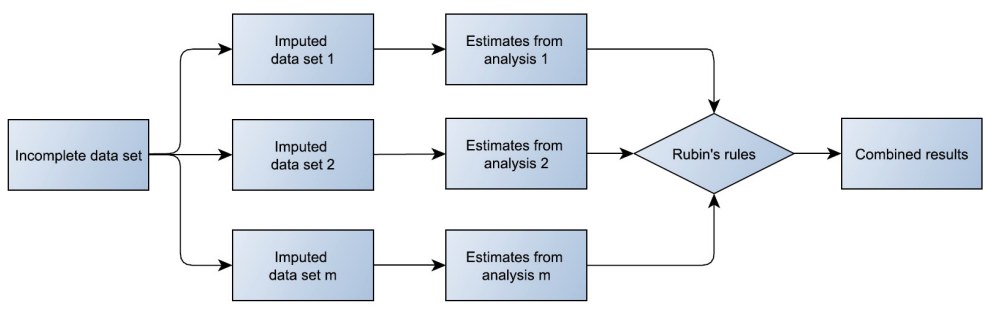
\includegraphics[width=\textwidth]{Images/Mice.png}
  \caption{The MICE-process \cite{wulff2017multiple}}
\end{figure}


Multiple imputations using chained equations or MICE is an imputation technique that uses multiple imputations to tackle missing data. MICE has become one of the principal methods of addressing missing data \cite{azur2011multiple}. Creating multiple imputations, as opposed to single imputations, accounts for the statistical uncertainty in the imputations. 

Since each variable is imputed using its own imputation model, MICE can handle different
variable types (for example, continuous, binary, categorical), as well as complexities such as varying bounds \cite{wulff2017multiple}. Multiple imputations (MI) was originally designed to handle missing data in public-use large datasets. Hence this is an ideal imputation technique for our data. 
Because multiple imputations involve creating multiple predictions for each missing value, the analysis of multiple imputed data take into account the uncertainty in the imputations and yield accurate standard errors \cite{wulff2017multiple}. 
% To carry out MICE, a series of regression models are run whereby each variable with missing data is modelled conditional upon the other variables in the data. This means that each variable can be modelled according to its distribution. For example, binary variables modelled using logistic regression and continuous variables modelled using linear regression.

We outline the MICE algorithm for a set of variables, $x_1 \dots x_k$, some or all of which have missing values. Initially, all missing values are filled in at random. The first variable with at least one missing value, $x_1$ say, is then regressed on the other variables, $x_2 \dots x_k$. The estimation is restricted to individuals with observed $x_1$. Missing values in $x_1$ are replaced by simulated draws from the posterior predictive distribution of $x_1$, an important step known as proper imputation. The next variable with missing values, say $x_2$, is regressed on all the other variables, $x_1, x_3, . . . , x_k$. Estimation is restricted to individuals with observed $x_2$ and uses the imputed values of $x_1$. Again, missing values in $x_2$ are replaced by draws from the posterior predictive distribution of $x_2$. The process is repeated for all other variables with missing values in turn: one such round is called a cycle. To stabilize the results, the procedure (similar to a Gibbs sampler) is usually repeated for about ten cycles to produce a single imputed dataset. The entire procedure is repeated independently `m' times, yielding `m' imputed data-sets. Standard texts on MI suggest that small numbers of imputed data-sets (m = 3 to 5) are adequate.


According to \cite{shrive2006dealing}, which does an extensive comparison between different imputation methods, multiple imputations is the most accurate method for dealing with missing data in most of the missing data scenarios.
The paper recommends using no more than M=5 imputations and sometimes as small number as 2 or 3 to generate useful statistical inferences. 

We carried out MICE imputation using python's \textit{fancyimpute} library and used 5 imputations in our study. 


\subsection{Dealing with Data Imbalance}
\label{sec:imbalance}
As bankruptcy is an uncommon event, it would be reasonable to note that there are only a few companies that file bankruptcy every year. We showcase this class imbalance on our own data in \autoref{table:Data organization and Instances}.

% to have a very small proportion companies in the public domain file for bankruptcy. This imbalance is evident in the dataset and is showcased in \autoref{table:Data organization and Instances}

Having an imbalanced dataset can cause our machine learning models to overfit to the majority class, i.e., companies that are still operational, i.e. non-bankrupt companies. Since the data is skewed towards one class, machine learning models can struggle to learn to correctly classify a minority class (bankrupt) instance. 
Despite this class imbalance, most models would still produce a reasonably high accuracy as most instances fall under the non-bankrupt majority class. Therefore, we disregard accuracy as a valid metric and use AUC, F1-Score, precision and recall, to evaluate the performance of our model.

To tackle this data imbalance, we use the over-sampling technique that has been proposed in \cite{le2018cluster}, to generate synthetic data that adds instances from the minority class to the dataset. This technique will raise the percentage of minority class data from around 5\% to 15\% of the dataset, as recommended by extensive work done in \cite{cao2013integrated}. This will allow the models to be exposed to a greater number of instances with the minority class, thus improving the chances for the model to predict the correct classification when an instance is labelled as bankrupt.

% In order to balance the dataset to improve the performance of the models used, we have used an oversampling technique called Synthetic Minority Over Sampling (SMOTE). The implementation and further details of this is discussed in \autoref{sec:SMOTE} 

Synthetic Minority Over-sampling Technique (SMOTE) is an algorithm has been used to over-sample the dataset as it is one of the most well-known techniques for oversampling. SMOTE \cite{chawla2002smote} works by selecting/sampling similar instances of the minority class, by finding the nearest neighbours $k$ (using Euclidean distance) and changing each attribute one at a time by multiplying each $x$ by a random number (between 0 to 1), therefore creating a new synthetic instance. We generate these minority class samples for our dataset after estimating the missing values using the previously mentioned imputation techniques. SMOTE has been implemented using the \textit{imblearn.over\_sampling} library.


\begin{table}[h!]
% \sm
\begin{center}
 \begin{tabular}{|l|p{2cm}|p{3cm}|p{3cm}|p{3cm}|} 
 \hline
 Dataset & Total number of instances & Number of bankrupt instances & Number of non-bankrupt instances & Percentage of bankrupt instances

  \\ [0.5ex] 
 \hline\hline
 
Year 1 & 2342 & 90 & 2252 & 3.93\% \\ \hline
 
Year 2 & 3391 & 134 & 3257 & 4.71\% \\ \hline
 
Year 3 & 3501 & 165 & 3336 & 5.25 \% \\ \hline
 
Year 4 & 3264 & 172 & 3092 & 6.93\% \\ \hline
 
Year 5 & 1970 & 137 & 1833 & 3.93\% \\ \hline

\end{tabular}
\end{center}

    \caption{Data organisation and Instances}
\label{table:Data organization and Instances}
\end{table}

\subsection{Dimensionality Reduction and Feature Selection}

Dimensionality reduction is a crucial component of financial analysis and has received a lot of interest in recent studies \cite{cao2012aggregating}. Many dimensionality reduction methods have been proposed, such as t-testing, correlation matrices, factor analysis, principal component analysis (PCA), independent component analysis (ICA), etc.
In a linear pre-processing stage, PCA and ICA are capable of improving the discriminating power of classifiers \cite{chen2009bankruptcy}. 
However, nonlinear projection methods are particularly applicable to solve high-dimensional financial data. Reducing the number of variables was found to be one of the key components in the successful prediction of bankruptcy, not only simplifying the model structure but also by improving the discriminative power \cite{cao2012aggregating}. The dimensionality reduction method we used is described in \autoref{sec:pca}

Feature selection techniques are methods used to eliminate features which are redundant or irrelevant. This is achieved using different methods; the most common is to find those features that are correlated to each other (or correlation with the outcome) thus removing redundant and unwanted features. 
% This in turn can simplify the hypothesis in a model which can improve both performance and memory allocation, while also reduces overfitting (reducing bias). 
Reducing the number of irrelevant or redundant features drastically reduces the running time of a learning algorithm and yields a more general concept. There are many potential benefits of feature selection, some of which are:
\begin{enumerate}
    \item Facilitating data visualisation and data understanding
    \item Reducing the measurement and storage requirements
    \item Reducing training and utilisation  times
    \item Defying the curse of dimensionality to improve prediction performances by simplifying the hypothesis in a model
\end{enumerate}

In addition, this helps in getting a better insight into the underlying concept of a real-world classification.
There are various techniques to achieve this, but for the purpose of this project, Recursive Feature Elimination (RFE) and Chi-Square feature selection will be described in \autoref{sec:RFE} and \autoref{sec:chi2} respectively.

\subsubsection{Principal Component Analysis (PCA)}
\label{sec:pca}
Dimensionality Reduction in our project was carried out using principal component analysis (PCA).
PCA re-orients a data set in the direction of the eigenvectors, which are ordered according to the extent of variance they capture from the data. The more eigenvectors we use, the higher the variance captured. PCA is a distributed representation wherein raw variables collaborate to generate a principle component. In predictive machine learning, principle components can replace the original variables. The objective is to learn the functional relationship between the target variable and the principle component. This can simplify the learning task, increase predictive accuracy, and facilitate feature reduction. 

\begin{figure}[htp]
\centering
\captionsetup{justification=centering}
  
  \centering
    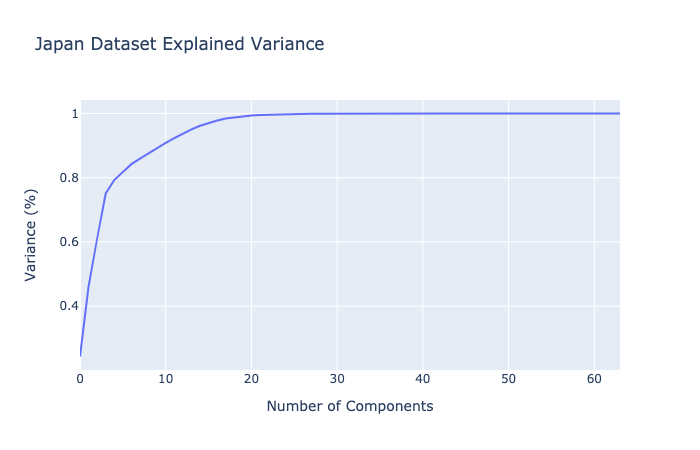
\includegraphics[width=\textwidth]{Images/pca.png}
  \caption{PCA Carried out on MICE Imputed and Oversampled Year-1 dataset.}
  \label{fig:pca}
\end{figure}

\autoref{fig:pca} shows the results of PCA being carried out on our dataset. After examining the graph, we decided to choose twenty, as the number of components as this seemed as the elbow point in the graph. Using just twenty components, we were able to attain a variance of 99.35\%.  

% \todo[inline]{New explaination}
% \textbf{COVID19-Note:} 
% The experimentation process required us to use Edinburgh University GPU's and work from DICE computers. Due to the closure of Appleton Tower on $17^{th}$ March 2020 and the inability to access University servers for computational needs, ongoing experiments using PCA was halted abruptly.
% Moving away from Edinburgh lead to further disruptions with connectivity and the change of environment demanded the need to prioritise writing the report. All further experiments were stopped due to the lack of adequate computational capacity.


\subsubsection{Recursive Feature Elimination}
\label{sec:RFE}
The Recursive Feature Elimination \cite{guyon2002gene}, as the name suggests, recursively fits the model and eliminates the least important feature/s with every iteration. This is done by ranking the features according to their coefficient weight and eliminating the least weighted features. After each iteration, the model has fitted again, and the least weighted feature/s are eliminated again until the specified number of maximum iterations or features to be eliminated is reached. In this project, the Logistic Regression classifier is used as an estimator.

The number feature selected from Recursive Feature Elimination was limited to 20, to maintain comparability with the dimensionality reduction methods.

The top 20 features selected by Recursive Feature Elimination are as follows: \\
'x11', 'x33', 'x52', 'x53', 'x61', 'x63', 'x13', 'x17', 'x19', 'x36', 'x54', 'x64', 'x6', 'x9', 'x23', 'x31', 'x32', 'x50', 'x8', 'x20'.

% \textbf{COVID19-Note:} Detailed experiments were not carried out using Chi-Square due to the lack of time and the difference seen in final results. Experimentation was halted and focus was readjusted to account new time-scale and lack of available computing resources.

\subsubsection{Chi-Square Feature Selection}
\label{sec:chi2}
The Chi-Square \cite{jin2006machine} is used to determine if the feature/s and outcome are dependent or not. The features and classes must not contain non-negative values (re-scaling is used to change negative values to positive values). It is often used in machine learning to rank features based on their Chi-Square statistic (score). Features that are found to be irrelevant for classification, are discarded depending on a specified number of features to be selected so that only the top-ranked features are selected.

Having normalised and re-scaled the data, the number feature selected from Chi-Square was limited to 20, to maintain comparability with the dimensionality reduction methods.

The top 20 features selected by Chi-Square are as follows: \\ 'x21', 'x27', 'x51', 'x32', 'x2', 'x44', 'x62', 'x43', 'x64', 'x30', 'x61', 'x52', 'x54', 'x53', 'x22', 'x58', 'x35', 'x20', 'x60', 'x47'.

\textbf{COVID19-Note:} 
The experimentation process required us to use Edinburgh University GPU's and work from DICE computers. Due to the closure of Appleton Tower on $17^{th}$ March 2020 and the inability to access University servers for computational needs, ongoing experiments using PCA, Recursive Feature Elimination and Chi-Square were halted abruptly.
Moving away from Edinburgh lead to further disruptions with connectivity and the change of environment demanded the need to prioritise writing the report. All further experiments were stopped due to the lack of adequate computational capacity.



